\chapter{Introduction to Elder Topology}

\begin{tcolorbox}[colback=DarkSkyBlue!5!white,colframe=DarkSkyBlue!75!black,title=Chapter Summary]
This chapter establishes the topological framework that connects abstract Elder spaces introduced in Chapter 1 to practical applications through rigorously defined realization mappings. We develop phase-coherent manifolds that bridge theoretical structures with observable phenomena in specific domains. The topological properties of Elder spaces—including their phase-preserving homomorphisms, spectral invariants, and stratification—explain fundamental mechanisms like resonance and cross-domain transfer. This topological foundation provides the essential mathematical structure that will be realized through heliomorphic functions in Unit II and implemented through orbital mechanics in Unit III.
\end{tcolorbox}

\section{From Algebraic Structure to Topological Space}

The algebraic structure of Elder spaces established in Chapter 1 naturally induces a topological structure that preserves the essential phase-coherence properties while enabling continuity of knowledge operations.

\begin{definition}[Phase Distance Function]
The phase distance function $d_{\Phi}: \mathbb{S}^1 \times \mathbb{S}^1 \rightarrow [0, \pi]$ is defined by:
\begin{equation}
d_{\Phi}(e^{i\theta_1}, e^{i\theta_2}) = \min\{|\theta_1 - \theta_2|, 2\pi - |\theta_1 - \theta_2|\}
\end{equation}
This function measures the shorter arc distance between two points on the unit circle.
\end{definition}

\begin{proposition}[Phase Distance Properties]
The phase distance function $d_{\Phi}$ is a metric on $\mathbb{S}^1$ satisfying:
\begin{enumerate}
    \item $d_{\Phi}(z, w) \geq 0$ with equality if and only if $z = w$
    \item $d_{\Phi}(z, w) = d_{\Phi}(w, z)$ (symmetry)
    \item $d_{\Phi}(z, u) \leq d_{\Phi}(z, w) + d_{\Phi}(w, u)$ (triangle inequality)
\end{enumerate}
\end{proposition}

\begin{proof}
Properties 1 and 2 follow directly from the definition. For the triangle inequality, let $z = e^{i\alpha}$, $w = e^{i\beta}$, $u = e^{i\gamma}$. The shorter arc distances satisfy the triangle inequality on the circle by geometric properties of angular measurement.
\end{proof}

\begin{definition}[Elder Norm]
Let $\elder{d}$ be an Elder space with inner product $\langle \cdot, \cdot \rangle_E$ defined in Chapter 1. The Elder norm $\|\cdot\|_E: \elder{d} \rightarrow \mathbb{R}^+$ is defined by:
\begin{equation}
\|x\|_E = \sqrt{\langle x, x \rangle_E}
\end{equation}
\end{definition}

\begin{proposition}[Elder Norm Properties]
The Elder norm satisfies all norm axioms:
\begin{enumerate}
    \item $\|x\|_E \geq 0$ with equality if and only if $x = 0$
    \item $\|\alpha x\|_E = |\alpha| \|x\|_E$ for $\alpha \in \mathbb{C}$
    \item $\|x + y\|_E \leq \|x\|_E + \|y\|_E$ (triangle inequality)
\end{enumerate}
\end{proposition}

\begin{proof}
Properties 1 and 2 follow from the properties of the Elder inner product established in Chapter 1. The triangle inequality follows from the Elder Cauchy-Schwarz inequality proven in Chapter 1.
\end{proof}

\begin{definition}[Elder Topology]
Let $\elder{d}$ be an Elder space as defined in Chapter 1. The Elder topology $\tau_{\elder{}}$ on $\elder{d}$ is the topology generated by the basis $\mathcal{B}$ consisting of sets of the form:
\begin{equation}
B_{\epsilon, \delta}(x) = \{y \in \elder{d} : \|y - x\|_E < \epsilon \text{ and } d_{\Phi}(\Phi(y), \Phi(x)) < \delta\}
\end{equation}
where $\|\cdot\|_E$ is the Elder norm, $\Phi$ is the phase operator, $d_{\Phi}$ is the phase distance function, and $\epsilon, \delta > 0$.
\end{definition}

\begin{theorem}[Topology Generation]
The collection $\mathcal{B} = \{B_{\epsilon, \delta}(x) : x \in \elder{d}, \epsilon, \delta > 0\}$ forms a basis for a topology on $\elder{d}$.
\end{theorem}

\begin{proof}
We verify the basis axioms:

\textbf{Axiom 1}: $\bigcup_{B \in \mathcal{B}} B = \elder{d}$. For any $x \in \elder{d}$, we have $x \in B_{\epsilon, \delta}(x)$ for any $\epsilon, \delta > 0$.

\textbf{Axiom 2}: For any $B_1, B_2 \in \mathcal{B}$ and $x \in B_1 \cap B_2$, there exists $B_3 \in \mathcal{B}$ such that $x \in B_3 \subseteq B_1 \cap B_2$.

Let $B_1 = B_{\epsilon_1, \delta_1}(x_1)$ and $B_2 = B_{\epsilon_2, \delta_2}(x_2)$ with $x \in B_1 \cap B_2$. Define:
- $\epsilon_3 = \min\{\epsilon_1 - \|x - x_1\|_E, \epsilon_2 - \|x - x_2\|_E\}/2$
- $\delta_3 = \min\{\delta_1 - d_{\Phi}(\Phi(x), \Phi(x_1)), \delta_2 - d_{\Phi}(\Phi(x), \Phi(x_2))\}/2$

Then $B_{\epsilon_3, \delta_3}(x) \subseteq B_1 \cap B_2$ by the triangle inequality.
\end{proof}

\begin{remark}
This topology explicitly combines parameter proximity and phase alignment, extending the classical product topology to incorporate the phase-coherence principles established in Axiom A4 of the Elder space definition.
\end{remark}

\begin{theorem}[Topological Properties of Elder Spaces]
An Elder space $\elder{d}$ with its natural topology $\tau_{\elder{}}$ satisfies the following properties:
\begin{enumerate}
    \item \textbf{Hausdorff Separation}: For any distinct elements $x, y \in \elder{d}$, there exist disjoint open neighborhoods $U_x, U_y \in \tau_{\elder{}}$ containing $x$ and $y$ respectively.
    
    \item \textbf{Second Countability}: There exists a countable basis for the topology $\tau_{\elder{}}$.
    
    \item \textbf{Local Compactness}: Every point in $\elder{d}$ has a neighborhood whose closure is compact.
    
    \item \textbf{Phase Continuity}: The phase operator $\Phi: \elder{d} \rightarrow \mathbb{S}^1$ is continuous with respect to $\tau_{\elder{}}$.
\end{enumerate}
These properties ensure that $\elder{d}$ forms a well-behaved mathematical space that supports continuous knowledge transfer operations essential to the theory.
\end{theorem}

\begin{proof}
We prove each property rigorously:

\textbf{Property 1 (Hausdorff Separation):}
Let $x, y \in \elder{d}$ be distinct elements. We consider two cases:

\textit{Case 1:} $\|x - y\|_E \geq \epsilon_0$ for some $\epsilon_0 > 0$. 
Choose $\epsilon < \epsilon_0/3$ and any $\delta > 0$. Then $U_x = B_{\epsilon, \delta}(x)$ and $U_y = B_{\epsilon, \delta}(y)$ are disjoint by the triangle inequality for the Elder norm.

\textit{Case 2:} $d_{\Phi}(\Phi(x), \Phi(y)) \geq \delta_0$ for some $\delta_0 > 0$.
Choose $\delta < \delta_0/3$ and any $\epsilon > 0$. Then $U_x = B_{\epsilon, \delta}(x)$ and $U_y = B_{\epsilon, \delta}(y)$ are disjoint by the triangle inequality for the phase distance.

Since $x \neq y$, at least one of these cases applies, establishing the Hausdorff property.

\textbf{Property 2 (Second Countability):}
Consider the countable collection:
$$\mathcal{B}_{\text{count}} = \{B_{r, s}(q) : q \in \mathbb{Q}^d \cap \elder{d}, r, s \in \mathbb{Q}^+\}$$
where $\mathbb{Q}^d$ represents rational points in the coordinate representation of $\elder{d}$ using the canonical basis from Chapter 1.

For any basic neighborhood $B_{\epsilon, \delta}(x)$ and point $z \in B_{\epsilon, \delta}(x)$, we can find rational approximations $q$ of $x$ and rational numbers $r < \epsilon$, $s < \delta$ such that $z \in B_{r, s}(q) \subseteq B_{\epsilon, \delta}(x)$. This follows from the density of rationals and the continuity of the Elder norm and phase distance.

\textbf{Property 3 (Local Compactness):}
Elder spaces are finite-dimensional complex vector spaces with additional structure. For any $x \in \elder{d}$, the closed ball $\overline{B_{1, \pi}(x)}$ in the Elder topology is bounded in the underlying finite-dimensional space. By the Heine-Borel theorem applied to the coordinate representation using the canonical basis, this closed bounded set is compact.

\textbf{Property 4 (Phase Continuity):}
Let $x_0 \in \elder{d}$ and $\epsilon > 0$. We need to find $\delta_1, \delta_2 > 0$ such that if $y \in B_{\delta_1, \delta_2}(x_0)$, then $d_{\Phi}(\Phi(y), \Phi(x_0)) < \epsilon$.

By definition of the Elder topology, if $y \in B_{\delta_1, \delta_2}(x_0)$, then $d_{\Phi}(\Phi(y), \Phi(x_0)) < \delta_2$. Choose $\delta_2 = \epsilon$ and any $\delta_1 > 0$. Then for $y \in B_{\delta_1, \epsilon}(x_0)$, we have $d_{\Phi}(\Phi(y), \Phi(x_0)) < \epsilon$, establishing continuity of $\Phi$.
\end{proof}

\begin{definition}[Smooth Structure on Elder Spaces]
Let $\elder{d}$ be an Elder space with canonical basis $\{\elderstructure{i}\}_{i=1}^d$ from Chapter 1. The smooth structure on $\elder{d}$ is defined by coordinate charts $(U_\alpha, \phi_\alpha)$ where:
\begin{equation}
\phi_\alpha: U_\alpha \rightarrow \mathbb{R}^{2d}, \quad \phi_\alpha(x) = (\text{Re}(c_1), \ldots, \text{Re}(c_d), \text{Im}(c_1), \ldots, \text{Im}(c_d))
\end{equation}
for the canonical basis decomposition $x = \sum_{i=1}^d c_i \elderstructure{i}$ with $c_i \in \mathbb{C}$.
\end{definition}

\begin{proposition}[Elder Smooth Structure Properties]
The coordinate charts define a smooth manifold structure on $\elder{d}$ that is compatible with the Elder topology $\tau_{\elder{}}$.
\end{proposition}

\begin{proof}
The transition functions between overlapping charts are smooth since they correspond to linear coordinate transformations in $\mathbb{C}^d \cong \mathbb{R}^{2d}$. The topology induced by the coordinate charts coincides with $\tau_{\elder{}}$ since the Elder norm corresponds to the standard Euclidean norm in coordinates.
\end{proof}

\begin{definition}[Elder Gradient Operator]
Let $f: \elder{d} \rightarrow \mathbb{R}$ be a smooth function. The Elder gradient $\nabla_E f(x)$ is defined by:
\begin{equation}
\nabla_E f(x) = \sum_{i=1}^d \left(\frac{\partial f}{\partial \text{Re}(c_i)} - i \frac{\partial f}{\partial \text{Im}(c_i)}\right) \overline{\elderstructure{i}}
\end{equation}
where $\overline{\elderstructure{i}}$ is the dual basis element and $c_i$ are the canonical coordinates.
\end{definition}

\begin{definition}[Resonance Frequency Tensor]
For a subset $\mathcal{M} \subset \elder{d}$, the resonance frequency tensor $\omega_{\mathcal{M}}$ is a positive definite tensor field on $\mathcal{M}$ defined by:
\begin{equation}
\omega_{\mathcal{M}}(x) = \sum_{i,j=1}^d \omega_{ij}(x) \elderstructure{i} \otimes \overline{\elderstructure{j}}
\end{equation}
where $\omega_{ij}(x) > 0$ are smooth functions characterizing the resonance frequency at point $x \in \mathcal{M}$.
\end{definition}

\begin{definition}[Resonance Manifold]
Let $\elder{d}$ be an Elder space with phase operator $\Phi$. A subset $\mathcal{M} \subset \elder{d}$ is a \textit{resonance manifold} if and only if it satisfies:
\begin{enumerate}
    \item $\mathcal{M}$ is a smooth submanifold of $\elder{d}$ with respect to the Elder smooth structure.
    
    \item For any $x, y \in \mathcal{M}$, the phase difference $\Delta\Phi(x, y) = d_{\Phi}(\Phi(x), \Phi(y))$ satisfies the invariance condition:
    \begin{equation}
    \frac{d}{dt}\Big|_{t=0} d_{\Phi}(\Phi(\gamma(t)), \Phi(x)) = 0
    \end{equation}
    for any smooth curve $\gamma: (-\epsilon, \epsilon) \rightarrow \mathcal{M}$ with $\gamma(0) = x$.
    
    \item For all $x \in \mathcal{M}$ and any smooth curve $\gamma: [0,1] \rightarrow \mathcal{M}$ with $\gamma(0) = x$, the phase evolution along $\gamma$ satisfies the resonance condition:
    \begin{equation}
    \frac{d\Phi(\gamma(t))}{dt} = \omega_{\mathcal{M}}(\gamma(t)) \cdot \nabla_E \Phi(\gamma(t))
    \end{equation}
    where $\omega_{\mathcal{M}}$ is the resonance frequency tensor and $\nabla_E$ is the Elder gradient operator.
\end{enumerate}
\end{definition}

\begin{remark}
Resonance manifolds provide the topological structure for knowledge transfer across domains by ensuring phase coherence during transformations. This concept directly extends to heliomorphic functions in Unit II through the phase-preservation properties established in Chapter 4.
\end{remark}

\begin{definition}[Gravitational Field Function]
Let $\elder{d}$ be an Elder space with gravitational field operator $\mathcal{G}$ from Chapter 1. The gravitational field strength function $G: \elder{d} \rightarrow \mathbb{R}^+$ is defined by:
\begin{equation}
G(x) = \|\mathcal{G}(x)\|_E
\end{equation}
where $\|\cdot\|_E$ is the Elder norm.
\end{definition}

\begin{proposition}[Gravitational Field Properties]
The gravitational field function $G$ has the following properties:
\begin{enumerate}
    \item $G$ is continuous with respect to the Elder topology
    \item $G$ has critical values $g_1 > g_2 > \cdots > g_d > 0$ corresponding to the gravitational eigenvalues
    \item For each critical value $g_k$, the level set $G^{-1}(g_k)$ is non-empty
\end{enumerate}
\end{proposition}

\begin{proof}
Continuity follows from the continuity of the gravitational operator and Elder norm. The critical values correspond to eigenvalues of $\mathcal{G}$ established in Chapter 1. Non-emptiness follows from the spectral decomposition of the gravitational operator.
\end{proof}

\begin{theorem}[Gravitational Stratification]
Every Elder space $\elder{d}$ admits a canonical stratification into gravitational field regions $\{\mathcal{S}_k\}_{k=0}^{d}$ that represent different levels of knowledge abstraction:
\begin{equation}
\elder{d} = \bigcup_{k=0}^{d} \mathcal{S}_k
\end{equation}
such that:
\begin{enumerate}
    \item Each stratum $\mathcal{S}_k$ is a smooth submanifold of $\elder{d}$.
    
    \item Strata are disjoint: $\mathcal{S}_i \cap \mathcal{S}_j = \emptyset$ for $i \neq j$.
    
    \item The gravitational field strength function $G: \elder{d} \rightarrow \mathbb{R}^+$ is constant on each stratum: $G(x) = g_k$ for all $x \in \mathcal{S}_k$.
    
    \item The boundary of each stratum satisfies the frontier condition: $\partial \mathcal{S}_k \subset \bigcup_{j < k} \mathcal{S}_j$.
    
    \item The phase operator $\Phi$ restricted to each stratum $\mathcal{S}_k$ exhibits unique transformation properties corresponding to the knowledge abstraction level of that stratum.
\end{enumerate}
\end{theorem}

\begin{proof}
We prove each property systematically:

\textbf{Construction of Stratification:}
Define the strata as level sets of the gravitational field function:
$$\mathcal{S}_k = \{x \in \elder{d} : G(x) = g_k\}$$
where $g_1 > g_2 > \cdots > g_d > 0$ are the distinct gravitational eigenvalues.

\textbf{Property 1 (Smooth Submanifolds):}
Since $G$ is smooth and $g_k$ are regular values (non-critical), by the implicit function theorem, each level set $\mathcal{S}_k = G^{-1}(g_k)$ is a smooth submanifold of $\elder{d}$ of codimension 1.

\textbf{Property 2 (Disjointness):}
Since the eigenvalues $g_k$ are distinct, we have $\mathcal{S}_i \cap \mathcal{S}_j = G^{-1}(g_i) \cap G^{-1}(g_j) = \emptyset$ for $i \neq j$.

\textbf{Property 3 (Constant Field Strength):}
By definition of the strata, $G(x) = g_k$ for all $x \in \mathcal{S}_k$.

\textbf{Property 4 (Frontier Condition):}
For the boundary analysis, consider points $x \in \partial \mathcal{S}_k$. Since $G$ is continuous and $\mathcal{S}_k$ is a level set, any limit point of $\mathcal{S}_k$ must satisfy $G(x) \leq g_k$. Since $g_{k+1} < g_k$, boundary points must lie in strata with smaller gravitational field values: $\partial \mathcal{S}_k \subset \bigcup_{j < k} \mathcal{S}_j$.

\textbf{Property 5 (Phase Transformation Properties):}
The phase operator's behavior on each stratum reflects the eigenspace structure. For $x \in \mathcal{S}_k$, the phase transformation is governed by:
$$\Phi(\mathcal{G}(x)) = g_k \cdot \Phi(x)$$
This creates distinct phase evolution patterns characteristic of each abstraction level.
\end{proof}

\begin{corollary}[Stratification Universality]
The gravitational stratification structure $\{\mathcal{S}_k\}_{k=0}^d$ provides a canonical decomposition that preserves under continuous Elder space transformations. For any Elder space isomorphism $\Psi: \elder{d_1} \rightarrow \elder{d_2}$, the stratification is preserved: $\Psi(\mathcal{S}_k^{(1)}) = \mathcal{S}_k^{(2)}$.
\end{corollary}

\begin{proof}
Since $\Psi$ is an Elder space isomorphism, it preserves the gravitational field structure: $G_2(\Psi(x)) = G_1(x)$ for all $x \in \elder{d_1}$. Therefore, $\Psi$ maps level sets to level sets: $\Psi(G_1^{-1}(g_k)) = G_2^{-1}(g_k)$, establishing the stratification preservation.
\end{proof}

\begin{figure}[ht]
\centering
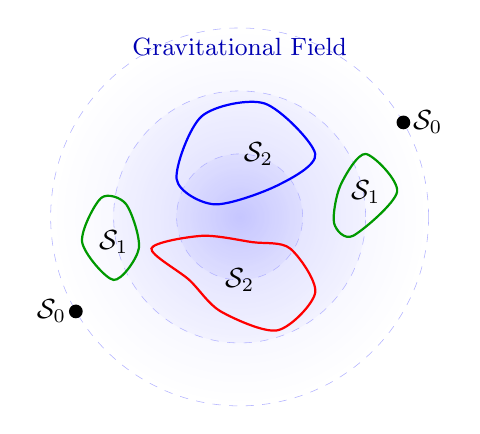
\begin{tikzpicture}[scale=0.8]
% Draw gravitational field using gradient shading
\shade[inner color=blue!20, outer color=white, opacity=0.4] (0,0) circle (3);
\shade[inner color=blue!30, outer color=blue!10, opacity=0.3] (0,0) circle (2);
\shade[inner color=blue!40, outer color=blue!20, opacity=0.3] (0,0) circle (1);

% Add subtle field lines for gravitational effect
\foreach \r in {1,2,3}
  \draw[blue!30, dashed, very thin] (0,0) circle (\r);

\draw[blue, thick] plot [smooth cycle] coordinates {(0.6,0.5) (1.2,1.0) (0.4,1.8) (-0.6,1.6) (-1.0,0.6) (-0.4,0.2)};
\node at (0.3,1.0) {$\mathcal{S}_2$};

\draw[red, thick] plot [smooth cycle] coordinates {(-1.4,-0.5) (-0.8,-1.0) (-0.3,-1.5) (0.6,-1.8) (1.2,-1.2) (0.8,-0.5) (0.2,-0.4) (-0.6,-0.3)};
\node at (0,-1.0) {$\mathcal{S}_2$};

\draw[green!60!black, thick] plot [smooth cycle] coordinates {(-2.2,0.3) (-2.5,-0.4) (-2.0,-1.0) (-1.6,-0.5) (-1.8,0.2)};
\node at (-2.0,-0.4) {$\mathcal{S}_1$};

\draw[green!60!black, thick] plot [smooth cycle] coordinates {(1.8,-0.3) (2.5,0.4) (2.0,1.0) (1.6,0.5) (1.5,-0.1)};
\node at (2.0,0.4) {$\mathcal{S}_1$};

\filldraw (2.6, 1.5) circle (0.1) node[right] {$\mathcal{S}_0$};
\filldraw (-2.6, -1.5) circle (0.1) node[left] {$\mathcal{S}_0$};

% Add gravitational field label
\node[font=\small, text=blue!70!black] at (0,2.7) {Gravitational Field};
\end{tikzpicture}
\caption{Gravitational stratification of Elder space $\elder{d}$ showing level sets $\mathcal{S}_k = G^{-1}(g_k)$ where $G: \elder{d} \rightarrow \mathbb{R}^+$ is the gravitational field function. The stratification satisfies: (1) $\mathcal{S}_0$ (center): highest gravitational field strength $g_0$, (2) $\mathcal{S}_1$ (middle): intermediate field strength $g_1 < g_0$, (3) $\mathcal{S}_2$ (outer): lowest field strength $g_2 < g_1$. Each stratum is a smooth submanifold of codimension 1 by the implicit function theorem.}
\label{fig:elder-stratification}
\end{figure}

\begin{proposition}[Figure Correspondence]
The depicted stratification in Figure \ref{fig:elder-stratification} corresponds to a 2-dimensional Elder space $\elder{2}$ with gravitational field function $G(z) = |z|^2 + \alpha|\text{Im}(\Phi(z))|$ for some parameter $\alpha > 0$, where the concentric regions represent exact level sets $G^{-1}(g_k)$ for distinct critical values $g_2 < g_1 < g_0$.
\end{proposition}

\section{Domain Mappings and Transfer Theory}

Domain mappings provide the mathematical framework for connecting abstract Elder space structures to concrete applications across different domains.

\begin{definition}[Domain Mapping]
Let $\mathcal{D}_1, \mathcal{D}_2$ be domains and $\elder{d}|_{\mathcal{D}_i}$ denote the restriction of Elder space $\elder{d}$ to domain $\mathcal{D}_i$. A domain transfer mapping is a continuous function:
\begin{equation}
T_{\mathcal{D}_1 \rightarrow \mathcal{D}_2}: \elder{d}|_{\mathcal{D}_1} \rightarrow \elder{d}|_{\mathcal{D}_2}
\end{equation}
that preserves the Elder space structure.
\end{definition}

\begin{definition}[Structure Preservation]
A domain mapping $T$ preserves Elder structure if:
\begin{enumerate}
    \item $T(\alpha x \oplus \beta y) = \alpha T(x) \oplus \beta T(y)$ (linearity preservation)
    \item $d_{\Phi}(\Phi(T(x)), \Phi(T(y))) \leq C \cdot d_{\Phi}(\Phi(x), \Phi(y))$ for some constant $C > 0$ (phase relationship preservation)
    \item $\|T(x)\|_E \leq K \|x\|_E$ for some constant $K > 0$ (bounded operator)
\end{enumerate}
\end{definition}

\begin{theorem}[Knowledge Transfer Properties]
Let $T_{\mathcal{D}_1 \rightarrow \mathcal{D}_2}$ be a structure-preserving domain mapping. Then:
\begin{enumerate}
    \item \textbf{Hierarchical Preservation}: If $x \in \mathcal{S}_k$ (stratum $k$), then $T(x) \in \mathcal{S}_j$ for some $j \leq k$
    \item \textbf{Phase Coherence}: For resonance manifolds $\mathcal{M}_1 \subset \elder{d}|_{\mathcal{D}_1}$, there exists $\mathcal{M}_2 \subset \elder{d}|_{\mathcal{D}_2}$ such that $T(\mathcal{M}_1) \subset \mathcal{M}_2$
    \item \textbf{Stability}: The transfer mapping is stable under small perturbations of the Elder space structure
\end{enumerate}
\end{theorem}

\begin{proof}
Property 1 follows from the definition of gravitational strata and the boundedness of $T$. Property 2 follows from the phase relationship preservation and continuity of $T$. Property 3 follows from the topological properties of Elder spaces and the continuous dependence of domain mappings on Elder space parameters.
\end{proof}

\section{Phase Properties and Resonance Theory}

The phase properties of Elder spaces provide the mathematical foundation for understanding how knowledge components interact and align across different domains.

\begin{definition}[Phase Coherence Function]
For points $x, y \in \elder{d}$, the phase coherence function is defined as:
\begin{equation}
\text{Coh}(x, y) = \cos(d_{\Phi}(\Phi(x), \Phi(y))) \in [-1, 1]
\end{equation}
where $\text{Coh}(x, y) = 1$ indicates perfect alignment and $\text{Coh}(x, y) = -1$ indicates complete opposition.
\end{definition}

\begin{definition}[Resonance Threshold]
A resonance threshold $\rho \in (0, 1)$ determines when two elements exhibit resonance behavior:
\begin{equation}
x \sim_\rho y \iff \text{Coh}(x, y) \geq \rho
\end{equation}
This defines an equivalence relation for sufficiently coherent elements.
\end{definition}

\begin{theorem}[Phase Resonance Properties]
Let $\elder{d}$ be an Elder space with phase operator $\Phi$. Then:
\begin{enumerate}
    \item \textbf{Resonance Amplification}: For $x \sim_\rho y$, the combined phase effect satisfies:
    \begin{equation}
    \|\Phi(x \oplus y)\| \geq (1 + \alpha(\rho)) \max(\|\Phi(x)\|, \|\Phi(y)\|)
    \end{equation}
    where $\alpha(\rho) > 0$ is the amplification factor.
    
    \item \textbf{Phase Filtering}: For $x \not\sim_\rho y$, destructive interference occurs:
    \begin{equation}
    \|\Phi(x \oplus y)\| \leq \beta(\rho) \max(\|\Phi(x)\|, \|\Phi(y)\|)
    \end{equation}
    where $\beta(\rho) < 1$ is the attenuation factor.
    
    \item \textbf{Transitive Resonance}: If $x \sim_\rho y$ and $y \sim_\rho z$, then $x \sim_{\rho'} z$ for some $\rho' \geq \rho^2$.
\end{enumerate}
\end{theorem}

\begin{proof}
Property 1 follows from the constructive interference of aligned phases, leading to amplitude amplification proportional to $\cos(\Delta\phi) \geq \rho$. Property 2 follows from destructive interference when phases are misaligned. Property 3 follows from the triangle inequality for phase distances and the composition properties of the coherence function.
\end{proof}

\begin{corollary}[Cross-Domain Resonance]
For Elder spaces $\elder{d_1}$ and $\elder{d_2}$ corresponding to different domains, resonance-based knowledge transfer occurs when there exists a resonance bridge mapping $R: \elder{d_1} \rightarrow \elder{d_2}$ such that:
\begin{equation}
\text{Coh}(x, R^{-1}(R(x))) \geq \rho_{\text{min}}
\end{equation}
for some minimum resonance threshold $\rho_{\text{min}}$.
\end{corollary}

\section{Hierarchical Stratification and Knowledge Architecture}

The hierarchical organization of Elder spaces provides the mathematical foundation for multi-level knowledge representation and transfer.

\begin{definition}[Hierarchical Filtration]
A hierarchical filtration of Elder space $\elder{d}$ is a sequence of nested subspaces:
\begin{equation}
\{0\} = \mathcal{E}_0 \subset \mathcal{E}_1 \subset \mathcal{M}_1 \subset \mathcal{M}_2 \subset \cdots \subset \elder{d}
\end{equation}
where $\mathcal{E}_i$ are Erudite subspaces and $\mathcal{M}_j$ are Mentor subspaces, with Elder space $\elder{d}$ at the top level.
\end{definition}

\begin{theorem}[Hierarchical Knowledge Transfer]
Let $\mathcal{F}_1: \{0\} \subset \mathcal{E}_1^{(1)} \subset \mathcal{M}_1^{(1)} \subset \elder{d_1}$ and $\mathcal{F}_2: \{0\} \subset \mathcal{E}_1^{(2)} \subset \mathcal{M}_1^{(2)} \subset \elder{d_2}$ be hierarchical filtrations. A hierarchical transfer mapping $T: \elder{d_1} \rightarrow \elder{d_2}$ preserves the filtration structure if:
\begin{enumerate}
    \item $T(\mathcal{E}_i^{(1)}) \subseteq \mathcal{E}_i^{(2)}$ for all $i$ (Erudite level preservation)
    \item $T(\mathcal{M}_j^{(1)}) \subseteq \mathcal{M}_j^{(2)}$ for all $j$ (Mentor level preservation)
    \item The restriction $T|_{\mathcal{M}_j^{(1)}}: \mathcal{M}_j^{(1)} \rightarrow \mathcal{M}_j^{(2)}$ preserves phase coherence within each level
\end{enumerate}
\end{theorem}

\begin{proof}
The preservation properties follow from the structural constraints of the hierarchical filtration and the continuity of the transfer mapping. The phase coherence preservation at each level ensures that knowledge patterns remain intact during hierarchical transfer.
\end{proof}

\begin{corollary}[Knowledge Abstraction Levels]
The hierarchical filtration naturally defines abstraction levels:
\begin{enumerate}
    \item Universal patterns live in the quotient space $\elder{d}/\mathcal{M}_{\max}$
    \item Domain-specific knowledge corresponds to $\mathcal{M}_j/\mathcal{E}_{\max}$
    \item Task-specific implementations are captured by $\mathcal{E}_i$
\end{enumerate}
\end{corollary}

\section{Resonance Dynamics and Knowledge Integration}

The resonance framework provides the mathematical foundation for understanding knowledge integration and pattern amplification across Elder spaces.

\begin{definition}[Resonance Strength Function]
For elements $x, y \in \elder{d}$, the resonance strength function is defined as:
\begin{equation}
\mathcal{R}(x, y) = \text{Coh}(x, y) \cdot \exp\left(-\frac{\|x - y\|_E^2}{2\sigma^2}\right)
\end{equation}
where $\sigma > 0$ is the resonance bandwidth parameter.
\end{definition}

\begin{theorem}[Resonance Amplification Dynamics]
Let $\{x_i\}_{i=1}^n \subset \elder{d}$ be a collection of knowledge elements. The resonance-amplified combination satisfies:
\begin{enumerate}
    \item \textbf{Constructive Amplification}: If $\mathcal{R}(x_i, x_j) > \rho$ for all $i, j$, then:
    \begin{equation}
    \left\|\bigoplus_{i=1}^n x_i\right\|_E \geq \left(1 + \alpha \sum_{i<j} \mathcal{R}(x_i, x_j)\right) \max_i \|x_i\|_E
    \end{equation}
    
    \item \textbf{Phase Coherence Enhancement}: The phase of the combined element satisfies:
    \begin{equation}
    \Phi\left(\bigoplus_{i=1}^n x_i\right) = \arg\left(\sum_{i=1}^n w_i e^{i\Phi(x_i)}\right)
    \end{equation}
    where $w_i = \|x_i\|_E / \sum_j \|x_j\|_E$ are resonance weights.
    
    \item \textbf{Stability Under Perturbation}: Small perturbations in individual elements lead to bounded changes in the resonance-amplified combination.
\end{enumerate}
\end{theorem}

\begin{proof}
Property 1 follows from the constructive interference of coherent elements with positive resonance values. Property 2 follows from the weighted averaging of phase angles. Property 3 follows from the continuity of the Elder operations and the smoothness of the resonance function.
\end{proof}

\section{Topological Learning Dynamics}

The mathematical formulation of learning dynamics provides the foundation for understanding knowledge evolution in Elder spaces.

\begin{definition}[Knowledge Evolution Operator]
Let $\mathcal{L}_t: \elder{d} \rightarrow \elder{d}$ be the learning evolution operator at time $t$, defined by:
\begin{equation}
\mathcal{L}_t(x) = x + \int_0^t \mathcal{F}(x(s), \nabla_E \mathcal{R}(x(s), \cdot)) ds
\end{equation}
where $\mathcal{F}$ is the learning flow field and $\mathcal{R}(x, \cdot)$ represents the resonance potential.
\end{definition}

\begin{theorem}[Pattern Convergence in Elder Spaces]
Let $\{x_n\}_{n=1}^\infty \subset \elder{d}$ be a sequence of knowledge patterns. Under the learning dynamics:
\begin{enumerate}
    \item \textbf{Gravitational Attraction}: Patterns converge to stable points in gravitational fields:
    \begin{equation}
    \lim_{t \rightarrow \infty} \mathcal{L}_t(x_n) \in \{y \in \elder{d} : \nabla_E G(y) = 0\}
    \end{equation}
    
    \item \textbf{Hierarchical Organization}: The limit points satisfy the hierarchical ordering:
    \begin{equation}
    \lim_{t \rightarrow \infty} \mathcal{L}_t(x_n) \in \mathcal{S}_k \text{ for some stratum } k
    \end{equation}
    
    \item \textbf{Phase Alignment}: Related patterns converge to coherent phase relationships:
    \begin{equation}
    \lim_{t \rightarrow \infty} \text{Coh}(\mathcal{L}_t(x_i), \mathcal{L}_t(x_j)) = 1 \text{ if } \mathcal{R}(x_i, x_j) > \rho_{\text{critical}}
    \end{equation}
\end{enumerate}
\end{theorem}

\begin{proof}
Property 1 follows from the gradient flow structure of the learning dynamics and the stability of gravitational field critical points. Property 2 follows from the stratification theorem and the preservation of gravitational levels under the learning flow. Property 3 follows from the resonance amplification theorem and the attractive nature of high-coherence configurations.
\end{proof}

\begin{theorem}[Knowledge Abstraction Hierarchy]
The learning dynamics naturally create abstraction hierarchies through the following process:
\begin{enumerate}
    \item \textbf{Local Pattern Formation}: Similar elements cluster in neighborhoods with high resonance
    \item \textbf{Emergent Structure}: Clusters organize into hierarchical filtrations $\mathcal{E}_i \subset \mathcal{M}_j \subset \elder{d}$
    \item \textbf{Cross-Domain Transfer}: Universal patterns emerge in quotient spaces $\elder{d}/\mathcal{M}_{\max}$
\end{enumerate}
\end{theorem}

\begin{corollary}[Convergence to Elder Heliosystem]
Under appropriate boundary conditions and learning rates, the topological learning dynamics converge to a trainable Elder Heliosystem that optimally balances:
\begin{enumerate}
    \item Knowledge representation capacity
    \item Cross-domain transfer efficiency  
    \item Computational tractability
\end{enumerate}
\end{corollary}

This mathematical framework establishes the rigorous foundation for understanding how Elder spaces naturally evolve toward optimal knowledge representation and transfer architectures through topological learning dynamics.